%\part*{Lezione 18/03/2021}
\subsubsection{Buca di potenziale} Riprendiamo il calcolo analitico della reazione di scattering tra protone e neutrone scegliendo per $u(r)$ e $u_S(r)$ una buca di potenziale. Partiamo dal deutone:
$$u(r) = \Biggl \{%
\begin{array}{ll}
    C_>e^{-\alpha r} & r>r_0  \\
    C_<\sin{k_0r} & r<r_0
\end{array}%
$$
con $\alpha \equiv \sqrt{mB_d}$ e $k_0\equiv \sqrt{m(V_0-B_d)}$ e i valori $r_0\simeq 2$ fm, $V_0 = 35$ MeV e $B_d \simeq 2.2$ MeV. 
Dalla continuità $C_> e^{-\alpha r_0} = C_<\sin{k_0r_0}$ e dalla normalizzazione:
\begin{displaymath}
\begin{aligned}
1 &= \int d^3r\: \ppc{\frac{u(r)}{r}}^2 \frac{1}{4\pi} = \int dr \: (u(r))^2 = \\
&= \int_0^{r_0} C_<^2\sin^2{k_0r} \: dr + \int_{r_0}^{+\infty} C_>^2 e^{-2\alpha r} \: dr =\\
&= C_<^2 \, \frac{r_0}{2} - \frac{\sin{2k_0r_0}}{2k_0} + C_>^2 \, \frac{e^{-2\alpha r_0}}{2\alpha}
\end{aligned}
\end{displaymath}
è possibile trovare le due costanti $C_>$ e $C_<$; riportiamo solo $C_>$:
$$C_> = \sqrt{\frac{2e^{2\alpha r_0}}{\frac{1}{\alpha} +\frac{1}{\sin^2{k_0r_0}}\ppc{r_0-\frac{\sin{2k_0r_0}}{2k_0}}}}$$
Per quanto riguarda invece l'onda di scattering:
$$\frac{u_S(r)}{r} = \Biggl \{%
\begin{array}{ll}
   \frac{1}{r}\, C^S_>\sin{(kr + \delta)} & r>r_0  \\
   \frac{1}{r}\, C^S_<\sin{k_1r} & r<r_0
\end{array}%
$$
con $\delta$ sfasamento, $k=\sqrt{mE}$ e $k_1\equiv\sqrt{m(E+V_0)}\to\sqrt{mV_0}$ per basse energie ($E\ll 1$). Dalla teoria dello scattering sappiamo che l'andamento asintotico per $r>r_0$ è $1-a_S/r$ dove $a_S$ è la lunghezza di scattering\index{lunghezza di scattering@$a_S$ lunghezza di scattering} che per il canale $\ce{^1S_0}$ è pari a circa $-24$ fm; la continuità impone quindi che 
$$\frac{C^S_{<}}{r_0}\sin{k_1r_0}=1-\frac{a_S}{r_0} \;\Rightarrow\; C^S_{<} = \frac{r_0 - a_S}{\sin{k_1r_0}}$$
Possiamo allora valutare l'integrale nell'espressione della sezione d'urto totale:
$$\int_0^{+\infty} dr \: u(r)u_S(r) = \int_0^{r_0} dr\: C_> \frac{e^{-\alpha r_0}}{\sin{k_0r_0}}\sin{k_0r}\,\, C_<^S \sin{k_1r}\:dr + \int_{r_0}^{+\infty} C_> e^{-\alpha r}(r-a_S) \: dr$$
$$\sigma = \frac{e^2}{v_{rel}}\frac{\mu^2_V q^3}{4m^2} \Bigl |\int_0^{+\infty} dr \, u(r) u_S(r)\Bigr |^2 \,\simeq\, 0.184\:\mbox{b}$$
Ricapitoliamo le approssimazioni fatte:
\begin{itemize}
    \item Abbiamo trascurato $\vec{J}_{conv}$.
    \item Abbiamo considerato solo l'onda $s$ nel deutone.
    \item $\mean{\vec{q}\cdot\vec{r}}\sim 0$ per cui $\exp{(i\vec{q}\cdot\vec{r})}\sim 1$.
    \item Abbiamo usato buche di potenziale per $u$ e $u_S$.
\end{itemize}
\subsubsection{Meson-Exchange Currents}
Osserviamo che il dato sperimentale $\sigma_{exp} \simeq 0.334$ b si discosta da quello teorico e ciò è dovuto appunto alle approssimazioni fatte, in particolare aver trascurato i termini di onda $d$ per il deutone. Nel calcolo della sezione d'urto, infatti, si ha un \textit{overlap} di due funzioni d'onda ${^3S_1}$ e ${^1S_0}$, che sono collegate allo stato di scattering del $pn$ e ortogonali perché corrispondono a stati differenti; è proprio questa ortogonalità che \vir{pompa} i termini piccoli\footnote{Questa situazione è simile a quella che avevamo incontrato per il decadimento $\beta$, quando avevamo fatto l'approssimazione di transizione permessa ($\phi_\nu^*\sim 1$).} come ${^3D_1}$
Tuttavia, questa approssimazione porta un contributo del 4\% ed è insolito che comporti un fattore 2 nel risultato; infatti anche rilasciando tutte quante le ipotesi fatte otteniamo $\sigma_{tot} \simeq 0.303$ b. La spiegazione di questa discrepanza di circa il 10\% è legata alle \textit{meson-exchange currents}\index{meson-exchange current@$J_{ij}^{MEC}$ \textit{meson-exchange current}}. Un'argomentazione \textit{na\"if} per descrivere il fenomeno consiste nello studio della corrente totale:
$$\vec{J}(\vec{q}) = \sum_i (\vec{J}_{C,i} + \vec{J}_{M,i})$$
dove la sommatoria è estesa prima al caso in cui l'interazione è tra fotone e protone con neutrone spettatore e successivamente tra fotone e neutrone con protone spettatore. Abbiamo quindi trascurato l'interazione nucleare tra protone e neutrone durante il processo, che interpretiamo come uno scambio di mesoni (tipo pioni $\pi$); il fotone può allora interagire con il pione carico $\pi^\pm$ e questo porta un termine di corrente a due corpi\footnote{Fu ipotizzata per la prima volta proprio nella risoluzione di questo problema.} $\vec{J}_{ij}^{MEC}$\footnote{$MEC$ sta appunto per \textit{meson-exchange current}.} nella corrente totale, contribuendo a fornire per la sezione d'urto teorica un valore pari a $0.333$ b.\\
Un metodo più rigoroso per mostrare la necessità di questo termine si sviluppa dalla conservazione della carica:
$$\Div{J}+\dt{\rho} = 0$$
dove $\rho = \rho_1 + \rho_2$ e $\vec{J}(\vec{x}) = \int \vec{J}(\vec{q})\:\exp{(-i\vec{q}\cdot\vec{x})}\,d^3q$. Ricordando che la derivata temporale è legata al commutatore con l'hamiltoniana e osservando che $\Div{J}\,\Rightarrow\,\vec{q}\cdot\vec{J}(\vec{q})$ allora si ha:
$$\vec{q}\cdot\vec{J}(\vec{q}) \propto \comham{\rho}$$
con $H = T+V_{12}$\footnote{Ricordiamo che %
$$T=\sum_{i=1}^2 \frac{p_i^2}{2m}$$%
}.
\begin{displaymath}
\begin{aligned}
\vec{q}\cdot\vec{J}&\propto \commute{T+V_{12}}{\rho_1+\rho_2} = \\
&= \commute{T}{\rho_1+\rho_2} + \commute{V_{12}}{\rho_1+\rho_2}
\end{aligned}
\end{displaymath}
Se non si considera un termine di accoppiamento nell'espressione della corrente è possibile mostrare che il prodotto scalare a sinistra è proporzionale solo al commutatore dell'energia cinetica; ciò implica necessariamente che debba esistere $\vec{q}\cdot\vec{J}_{12}^{MEC}\propto\commute{V}{\rho}$ e dalle osservazioni intuiamo che debbano valere tra 0.30 e 0.33.
\newpage
\subsection{Una parentesi: Metodo \textit{ab-initio}}\label{0318-sec-abinitio}\index{Metodo ab-initio@Metodo \textit{ab-initio}} Riassumiamo tutto quello che abbiamo fatto:
\begin{enumerate}[1]
    \item Studio della cinematica $\to$ Integrale $\psi_i,\psi_f,\vec{J}$.
    \item Calcolo delle funzioni d'onda $\to$ Necessario conoscere $V_{12}$ e un metodo numerico accurato per risolvere l'equazione di \Sch.
    \item Considerare un modello \vir{realistico} per $\vec{J}$ $\to$ Introdurre il termine di corrente a due corpi $\vec{J}^{MEC}_{ij}$.
    \item Risultato $\to$ Ottengo una predizione per $\sigma$.
\end{enumerate}
Questo metodo che parte da un'espressione del potenziale e della corrente conosciuta e ben testata e permette di ricavare una predizione viene definito \textit{ab-initio}\index{Metodo ab-initio@Metodo \textit{ab-initio}}.\\
Consideriamo ora un problema a 2 corpi con 3 nucleoni ($A=3$), per esempio:
$$p+d\to \ce{^3He}+\gamma$$
Come anticipato la cinematica è la stessa dello \textit{scattering} $pn$, ma in questo caso abbiamo difficoltà nel calcolo dell'espressione per $V_{12}$, infatti si ha una differenza di circa 1 MeV tra l'energia di legame attesa e quella misurata del $\ce{^3He}$\footnote{Nello specifico: $B(\ce{^3He})\sim6.5\div 6.9$ MeV contro il valore osservato $B^{oss}(\ce{^3He})\sim7.75$ MeV.%
}. Per risolvere questa discrepanza è necessario introdurre un termine di interazione a 3 corpi $V_{123}$\footnote{Non si risolve comunque totalmente le difficoltà, dal momento che, nonostante i modelli siano studiati sin dagli anni '50, tuttora il campo dell'interazione a 3 corpi è un ambito di ricerca ancora aperto.}, ma rimane comunque l'equazione di \Sch{} le cui soluzioni per $A=3$ non sono semplici. Proprio questo è il difetto del metodo \textit{ab-initio}\index{Metodo ab-initio@Metodo \textit{ab-initio}}: è limitato dalle tecniche numeriche per il calcolo di $\psi_{in}$ e $\psi_{out}$. Nel caso di $A=3$, come il nostro, esiste un metodo inventato a Pisa detto \textit{Metodo delle Armoniche Ipersferiche}\complementi{Metodo delle Armoniche Ipersferiche}, che permette anche di lavorare con $A=4$ e si sta sviluppando per raggiungere $A=6$.\\
Per quanto riguarda la corrente, avremo anche un termine a 3 corpi:
$$\vec{J} = \sum_i \vec{J}_i + \sum_{i<j} \vec{J}_{ij} + \sum_{i<j<k} \vec{J}_{ijk}$$
fortunatamente questo termine, per cui esiste un metodo di sviluppo, non contribuisce particolarmente al risultato.\\
I metodi \textit{ab-initio}\index{Metodo ab-initio@Metodo \textit{ab-initio}}, quindi, sono generali e non necessitano di \vir{aggiustare} valori per ottenere le corrette relazioni, tuttavia richiedono una struttura teorica alla base che diviene sempre più complessa al crescere di $A$\footnote{Vedremo nei capitoli successivi altri metodi per questi casi.}. 



\chapter{La catena protone-protone}\label{cap-pp}

\paragraph{Introduzione} Dopo questa breve digressione torniamo alla BBN\index{Big Bang Nucleosynthesis}: a circa $4\cdot\ord{5}$ anni dal \textit{Big Bang} l'energia degli elettroni è abbastanza bassa ($T\sim\ord{3}$ K ovvero $kT\sim0.1$ eV) per legarsi in atomi e questo segna il disaccoppiamento dalla radiazione e la nascita del CMB\index{Cosmic Microwave Background@Cosmic Microwave Background CMB}; successivamente a $\ord{9}$ anni dal \textit{Big Bang} si ha la formazione delle prime stelle e galassie. A questo punto ci concentreremo sulla nucleosintesi stellare.

\paragraph{Dentro il Sole: alcuni valori}\complementi{Valori solari}
\begin{itemize}
    \item $T_{sup}\sim 6000\unit{K}$
    \item $T_{int}\sim 1.5\cdot\ord{7}\unit{K}$
    \item $R\sol\sim 7\cdot\ord{8}\unit{m}$
    \item $M\sol\sim 2\cdot\ord{30}\unit{kg}$
    \item $L\sol\sim 3.8\cdot\ord{26}\unit{W}$
    \item $X\sim 70\%$, $Y\sim 29\%$, $Z\sim 1\%$\footnote{Con $X,Y,Z$ si intende rispettivamente la frazione su massa di idrogeno, di elio e la metallicità\index{metallicità}}.
\end{itemize}
\acc{E} necessario \vir{invocare} la nucleosintesi perché la sola energia gravitazionale non è sufficiente a sostenere la struttura per le quantità di tempo osservate, infatti si avrebbe:
$$\tau\sol^g = \frac{\text{Energia disponibile}}{L\sol} \simeq \frac{3}{5}\frac{GM\sol^2}{R\sol\:L\sol }\sim 2\cdot\ord{7}\unit{y}\ll\tau\sol^{oss}$$
Usando per esempio la $4p\to\ce{^4He}$ detta appunto \textbf{catena protone-protone}\index{Catena protone-protone@Catena protone-protone $pp$} si ha un'energia rilasciata legata alla differenza di massa: $\Delta m = 4m_p - m_{\ce{He}} \simeq 4\cdot(1.0078\unit{u})-4.0026\unit{u} = 0.029\unit{u}\simeq 0.7\%$ della massa iniziale, per cui
$$\tau\sol^{pp}\sim\frac{0.007\cdot0.1\mbox{M}\sol c^2}{L\sol}\simeq \ord{10}\unit{y} \;\text{ordine di } \tau\sol^{oss}$$
dove abbiamo supposto che il 10\% della massa solare venga fusa.

\section{Una prima occhiata}
In termini puramente energetici:
$$\Delta m c^2 = (4m_p - m_{\ce{He}})c^2 \simeq 4\cdot 938.3 - 2\cdot 938.3 \,-\, 2\cdot 939.6 + \underbrace{B_{\ce{He}}}_{28} \sim 26\unit{MeV}$$
Riportiamo in Figura \ref{0318_solnu} uno schema per la catena $pp$\index{Catena protone-protone@Catena protone-protone $pp$} con alcune delle varie diramazioni possibili.

\begin{figure}[h]
    \centering
    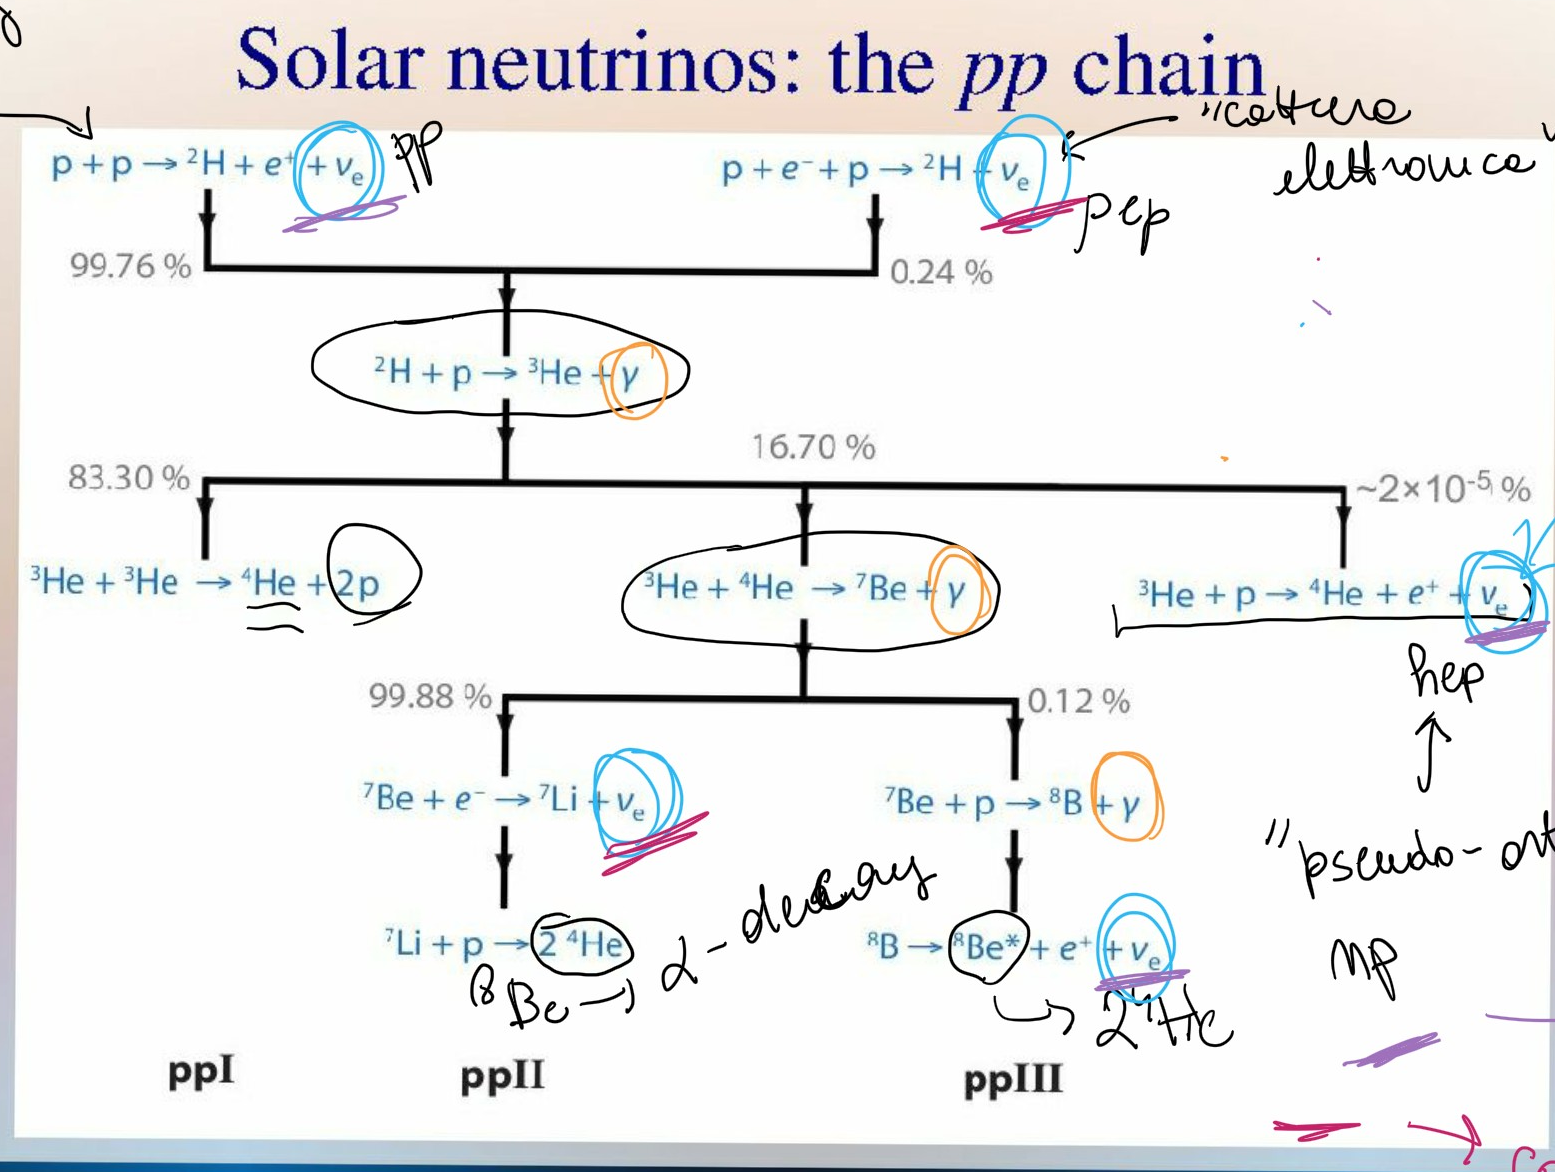
\includegraphics[scale=0.3
    ]{Immagini/0318_solarnu.png}
    \caption{Schema della catena protone-protone. In celeste sono stati cerchiati i neutrini prodotti, di cui quelli sottolineati in viola hanno spettro continuo, mentre quelli sottolineati in magenta hanno spettro a riga. In arancione sono cerchiati i fotoni prodotti. In nero sono cerchiati i decadimenti $\alpha$ del $\ce{^8Be}$.}
    \label{0318_solnu}
\end{figure}

\begin{itemize}
    \item \textbf{Prima reazione:} poiché non esiste uno stato legato per $p+p$ si ha prima un decadimento (tipo $\beta^+$) $p\to n$ e poi $p+n$. Osserviamo che la prima reazione è debole ed è un processo di cattura di 2 protoni\index{Catena protone-protone@Catena protone-protone $pp$!a@$pp$}. Esiste anche la possibilità di un'altra reazione, chiamata $pep$\index{Catena protone-protone@Catena protone-protone $pp$!b@$pep$}, $p+e^-+p$ che assomiglia a una cattura elettronica, ma essendo una reazione a 3 corpi è molto meno probabile della $pp$.
    \item \textbf{Seconda reazione:}\index{Catena protone-protone@Catena protone-protone $pp$!c@$dp$} in questo caso si ha una sola reazione possibile con interazione elettromagnetica, quindi si forma velocemente $\ce{^3He}$.
    \item \textbf{Canale $pp$I:}\index{Catena protone-protone@Catena protone-protone $pp$!e@$pp$I} intuitivamente si sarebbe portati a pensare che la reazione $\ce{^3He} + p$, detta $hep$\index{Catena protone-protone@Catena protone-protone $pp$!d@$hep$}, sia favorita dato che ci sono molti protoni e la barriera coulombiana è la più bassa, anche se è mediata dall'interazione debole; tuttavia questo non accade a causa dell'ortogonalità tra gli stati iniziale e finale (\textit{pseudo-ortogonalità} $np$\index{pseudo-ortogonalità@pseudo-ortogonalità $np$}), rendendo rilevanti i contributi dei termini agli ordini successivi.\\
    Nemmeno $\ce{^3He}+d$ va bene, perché questa ha $A=5$, per cui il primo canale della catena è quella che viene detta catena $pp$I\footnote{Il Sole ha bruciato finora principalmente con questo canale.}, ovvero $\ce{^3He}+\ce{^3He}$.
    \item \textbf{Reazioni successive:} a questo punto si ha una certa abbondanza di $^4He$ (prima troppo esigua) e si \vir{sblocca} così la reazione $\ce{^3He}+\ce{^4He}$ (che era presente anche nella BBN\index{Big Bang Nucleosynthesis}) con una probabilità di circa il 17\%. A questo punto ci sono due rami: una cattura o elettronica o radiativa.\\ 
    Il \textbf{canale $pp$II}\index{Catena protone-protone@Catena protone-protone $pp$!f@$pp$II} è mediato dall'interazione debole, tuttavia è più probabile del \textbf{canale $pp$III}\index{Catena protone-protone@Catena protone-protone $pp$!g@$pp$III} che è invece mediato dall'interazione elettromagnetica; ciò è dovuto alla differenza nella barriera di potenziale delle due reazioni.\\
    Infine, per quanto riguarda $\ce{^7Li + p}$ della $pp$II, in realtà questo è un processo in 2 step: $\ce{^7Li + p}\to\ce{^8Be}^*\to2\alpha$, dove l'ultimo decadimento è molto veloce.
\end{itemize} 
Indipendentemente dal ramo della catena si ha sempre la produzione di un $\alpha$ da $4p$.

\paragraph{Evidenze sperimentali} Ovviamente tale modello necessita di una verifica osservabile. I fotoni confermano la luminosità, ma non dimostrano la necessità della nucleosintesi; sono quindi i neutrini (il cui cammino libero nel Sole è maggiore delle sue dimensioni) le principali evidenze. In particolare, neutrini che derivano da differenti reazioni hanno energie diverse\footnote{I neutrini della $hep$, per esempio, sono i più energetici} e anche distribuzioni diverse\footnote{Quelli che compaiono come uno dei 3 corpi di un prodotto avranno spettro continuo, gli altri avranno una distribuzione a $\delta$.}. 


